\begin{frame}{application whitelisting}
\begin{itemize}
\item how about we only let standard applications run, unmodified?
    \begin{itemize}
    \item AppStore-based strategy?
    \end{itemize}
\item not uncommon in corporate environments:
\end{itemize}
\vspace{.5cm}
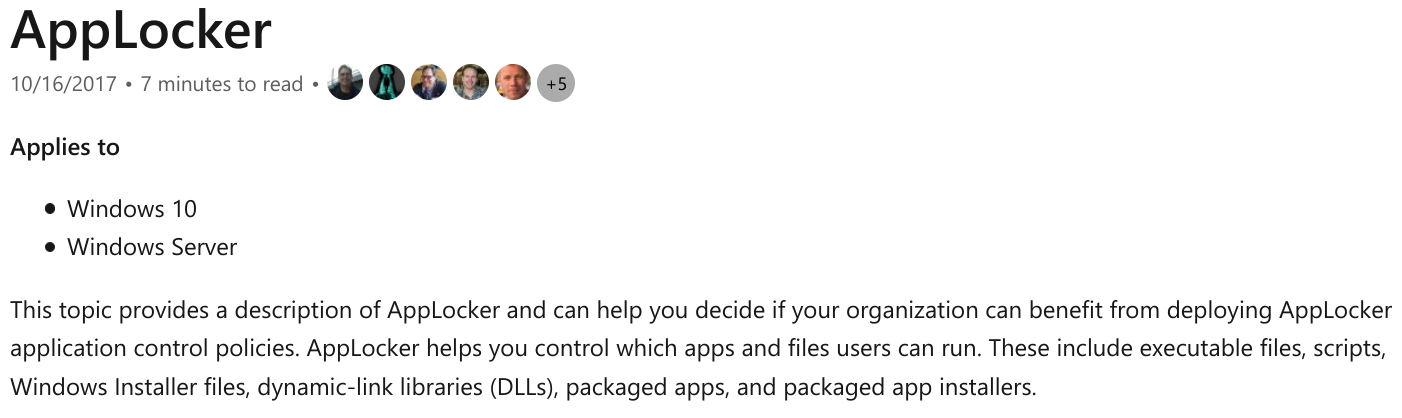
\includegraphics[width=\textwidth]{../heur-detect/applocker-manual}
\end{frame}

\begin{frame}{case study: Microsoft AppLocker}
    \begin{itemize}
    \item AppLocker is Windows 7+ feature for limiting what can run
        \begin{itemize}
        \item successor(?) feature App Control for Business (Windows 10+)
        \end{itemize}
    \item adminstrator sets rules about\ldots
    \item what publisher is allowed
        \begin{itemize}
        \item publisher cryptographically signs applications
        \item virus-like techniques break signatures
        \item allows upgrades!
        \end{itemize}
    \item what file hashes are allowed
        \begin{itemize}
        \item requires manual update each time software updates
        \end{itemize}
    \item what locations are allowed
        \begin{itemize}
        \item presumably for administrator-only directories
        \end{itemize}
    \end{itemize}
\end{frame}

\begin{frame}{problems with whitelisting}
    \begin{itemize}
    \item programs with features/bugs malware could exploit
        \begin{itemize}
        \item ``AppLocker does not control the behavior of applications after they are launched. Applications could contain flags passed to functions that signal AppLocker to circumvent the rules and allow another .exe or .dll to be loaded.''
        \end{itemize}
    \item users want to install/develop other software
    \item scripting:
        \begin{itemize}
        \item ``Not all host processes call into AppLocker and, therefore, AppLocker cannot control every kind of interpreted code''
        \end{itemize}
    \end{itemize}
\end{frame}
